% Configurazione
\documentclass{article}

\usepackage{titling} % Required for inserting the subtitle
\usepackage{graphicx} % Required for inserting images
\usepackage{tabularx} % Per l'ambiente tabularx (tabelle)
\usepackage{calc} % Sempre per le tabelle
\usepackage[hidelinks]{hyperref} % Per i collegamenti ipertestuali, ad esempio sulla table of contents
\usepackage{xcolor} % Per colorare il testo
\usepackage{colortbl} % Per colorare le celle delle tabelle
\usepackage{lipsum} % Per generare lorem ipsum
\usepackage[normalem]{ulem} % Per sottolineare il testo
\usepackage{array} % Per la visualizzazione fluttuante di array di domande e risposte
\usepackage{ragged2e} % Pacchetto necessario per \justifying che giustifica il testo di tabelle
\usepackage{placeins}

\newcommand{\ulhref}[2]{\href{#1}{\uline{#2}}} % Nuovo comando per sottolineare i link
\newcommand{\ulref}[1]{\uline{\ref{#1}}} % Nuovo comando per sottolineare i collegamenti a immagini
\setlength{\parindent}{0pt} % Rimuove il rientro automatico dei paragrafi

\graphicspath{ {immagini/} {../shared/images} }

% Struttura
\begin{document}
	\begin{minipage}{0.4\textwidth}
		
\includegraphics[width=0.6\textwidth]{logo_unipd}
	\end{minipage}
	\begin{minipage}{0.55\textwidth}
		\textcolor{red}{\textbf{Università degli Studi di Padova}} \\
		\textcolor{red}{Laurea: Informatica} \\
		\textcolor{red}{Corso: Ingegneria del Software} \\
		\textcolor{red}{Anno Accademico: 2025/2026}
	\end{minipage}
	
	\begin{minipage}{0.4\textwidth}
		
\includegraphics[width=0.6\textwidth]{logo_gruppo}
	\end{minipage}
	\begin{minipage}{0.55\textwidth}
		\textbf{Gruppo: NullPointers Group} \\
		Email: \textsf{nullpointersg@gmail.com}
	\end{minipage}
	
	\vspace{2cm}
	
	{
		\centering
		\Huge\bfseries Preventivo Costi\par
		\vspace{0.5cm}
	}
	
	\begin{center}
		\begin{tabular}{r|l}
			Stato & In Approvazione \\
			Versione & 0.2 \\
			Data ultima modifica & 26/10/2025 \\
			Destinatari & NullPointers Group \\
			& Prof. Tullio Vardanega \\
			& Prof. Riccardo Cardin \\
		\end{tabular}
	\end{center}
	
	\newpage
	\section{Registro delle modifiche}
	
	\begin{table}[htbp]
		\begin{tabular}{|c|c|c|c|c|}
			\hline
			\rowcolor[gray]{0.9}
			Vers & Data & Autore & Ruolo & Descrizione \\
			\hlineù
			0.3 & 27-10 & Matteo Mazzaretto & - & Miglioramento definizione amministratore  \\ 
			\hline
			0.2 & 26-10 & Tommaso Ceron & - & Aggiunta grafico impegni orari e suddivisione ruoli\\
			\hline
			0.2 & 24-10 & Laura Pieripolli & - & Continuazione stesura \\
			\hline
			0.1 & 24-10 & Matteo Mazzaretto & - & Creazione e stesura documento \\
			\hline
		\end{tabular}
	\end{table}
	
	\newpage
	
	\section{Scopo del documento}
	Questo documento ha lo scopo di illustrare ed identificare il nostro impegno, basandosi sulla nostra intensità e volontà, per il progetto.\\
	Elencheremo i nostri impegni orari, indicando anche un'analisi dei ruoli, concludendo con il preventivo del progetto e la data di consegna.\\
	%In base a quanto scritto, il gruppo sedicesimo NullPointers Group intende presentarsi per il seguente capitolato:\\
	\begin{center}
		
	\end{center}
	
	\section{Impegni orari}
	Dopo aver discusso tra i membri del gruppo, abbiamo definito le ore che ogni membro può dedicare al progetto.\\
	Ogni membro del gruppo si impegna a dedicare al progetto un totale di 90 ore produttive, ripartite equamente tra i ruoli di \textbf{Responsabile, Amministratore, Analista, Progettista, Programmatore} e \textbf{Verificatore}.\\
	Di seguito è riportata una tabella che riassume gli impegni orari di ogni ruolo:	
	
	\begin{table}[h!]
	\centering
	\begin{tabular}{|c|c|}
	\hline
	\rowcolor{gray!25}
	Ruolo & Ore \\ \hline
	Responsabile & 50  \\ \hline
	Amministratore & 40 \\ \hline
	Analista & 95  \\ \hline
	Progettista & 125 \\ \hline
	Verificatore & 105 \\ \hline
	Programmatore & 125 \\ \hline
	\end{tabular}
	\caption{Tabella dei costi relativa alle ore per ruolo}
	\end{table}

	\section{Analisi dei Ruoli}
		\subsection{Responsabile}
		Il Responsabile riveste un ruolo centrale nelle prime fasi del progetto, coordinando le attività del gruppo e garantendo una pianificazione efficace.
		Con l’avanzare del lavoro, il team acquisirà maggiore autonomia, mentre il Responsabile continuerà a svolgere funzioni di supervisione e controllo, assicurando il rispetto delle scadenze e la coerenza dei risultati con gli obiettivi prefissati.
		Sarà inoltre il principale punto di riferimento nelle comunicazioni tra il gruppo, i proponenti e i committenti.
		Trattandosi di un ruolo principalmente di "rappresentanza", abbiamo previsto di destinargli circa il 9\% delle ore totali.
		
		\subsection{Amministratore}
		L'Amministratore si occupa della configurazione e gestione dell'infrastruttura IT di supporto al progetto.
		Il suo ruolo è particolarmente importante nelle fasi iniziali e durante il deployment, dove raggiunge il picco di impegno per garantire un deploy corretto.
		Con il progredire del progetto, il suo contributo diminuisce man mano che i membri del gruppo diventano autonomi nell'uso degli strumenti predisposti.
		
		\subsection{Analista}
		L'analista è cruciale durante le fasi iniziali del progetto, si occupa di identificare e chiarire i requisiti, interpretando le esigenze degli utilizzatori finali per garantire una corretta definizione delle funzionalità.\\
		L'analisi viene svolta in collaborazione con l'azienda proponente e successivamente rielaborata dal gruppo che redirigerà il documento dei requisiti.\\
		Con l’avanzare del progetto, il monte ore dedicato a questo ruolo diminuirà, pur restando attivo per eventuali aggiornamenti o adattamenti dei requisiti in base al confronto con il proponente.
		
		\subsection{Progettista}
		Il progettista ha il ruolo di definire come un sistema dovrà funzionare, traducendo i requisiti in un'architettura software.
		Si occupa di seguire lo sviluppo, ma non la manutenzione.
		Con l'avanzare del progetto, il numero di ore previste per questo ruolo diminuirà, rimanendo ad ogni modo attivo per seguire eventuali aggiornamenti da parte del proponente.

		\subsection{Programmatore}
		Il programmatore è responsabile dello sviluppo del codice sorgente del progetto, traducendo il design in codice funzionante testabile dal proponente.\\
		Collabora attivamente con il progettista per assicurarsi che tutte le funzionalità siano implementate correttamente.

		Si stima un monte ore superiore alla media dovute alla necessità di integrare le numerose tecnologie che si andranno ad utilizzare.
		\subsection{Verificatore}
		Il Verificatore si occupa di assicurare la qualità dei prodotti e dei processi adottati, effettuando revisioni e test. 
		Questo ruolo richiede una presenza persistente per tutta la durata del progetto, in modo da poter seguire efficacemente tutte le fasi previste.
		
	
	\section{Preventivo costi}
	Di seguito è riportata una tabella contenente la ripartizione individuale nei vari ruoli, comprensiva del preventivo dei costi orari e totali.
	\begin{table}[h!]
	\centering
	\begin{tabular}{|c|c|c|c|}
	\hline
	\rowcolor{gray!25}
	Ruolo & Ore Totali & Costo (€/h) & Costo Totale (€) \\ \hline
	Responsabile & 50 & 30 & 1500 \\ \hline
	Amministratore & 40 & 20 & 800 \\ \hline
	Analista & 95 & 25 & 2375\\ \hline
	Progettista & 125 & 25 & 3125 \\ \hline
	Verificatore &  105 & 15 & 1575 \\ \hline
	Programmatore &  125 & 15 & 1875 \\ \hline
	\rowcolor{gray!25}
	& Ore tot.: 540  &  & Costo tot.: 11.250 \\ \hline
	\end{tabular}
	\caption{Impegni orari e ripartizione dei costi}
	\end{table}
	\FloatBarrier
	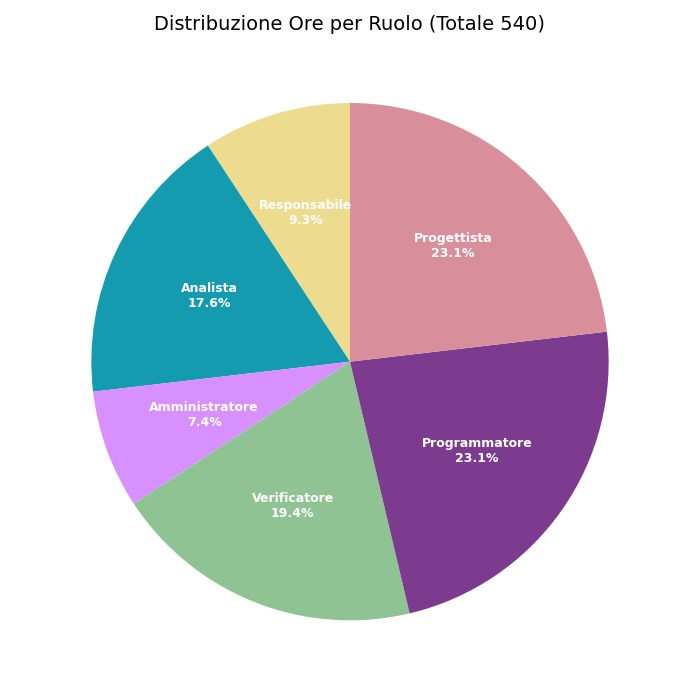
\includegraphics[width=1.0\textwidth]{grafico_costi.jpeg}
	Il costo finale calcolato in base alle tariffe orarie dei ruoli ed alle ore preventivate risulta di: 11.250€.
	
	\section{Data di consegna}
	Dopo le stime orarie e dei costi sopra riportati, il gruppo si impegna a terminare il progetto didattico entro il giorno 30/04/2026
	
	
	
\end{document}